% preamble %
\documentclass[12pt]{article}
\usepackage{amsfonts}
\usepackage{fancyhdr}
\usepackage{comment}
\usepackage[a4paper, top=1cm, bottom=1.5cm, left=2cm, right=2cm]{geometry}
\usepackage{enumitem}
\usepackage{times}
\usepackage{changepage}
\usepackage{amssymb}
\usepackage{graphicx}
\usepackage{tabularx}
\usepackage{titlesec}
\usepackage{hyperref}
\usepackage{changepage}
\usepackage[parfill]{parskip}
\usepackage{wrapfig}
\usepackage[export]{adjustbox}
\usepackage{multirow}
\usepackage{array}
\usepackage[table]{xcolor}
\usepackage{longtable,booktabs}
\usepackage{float}

% settings %
\setcounter{secnumdepth}{2} % enumerate
\setcounter{tocdepth}{2}    % TOC entries
%\renewcommand{\contentsname}{Innholdsfortegnelse}
\newcounter{frcounter}
\newcounter{frsubcounter}[frcounter]
\newcounter{nfrcounter}
\newcounter{nfrsubcounter}[nfrcounter]
\titlespacing*{\paragraph}{\parindent}{1ex}{1em}

% commands %
    % counters %
\newcommand*{\FR}{\stepcounter{frcounter}\textbf{[FR-\arabic{frcounter}] \quad}}
\newcommand*{\FRsub}{\stepcounter{frsubcounter}\textbf{[FR-\arabic{frcounter}.\arabic{frsubcounter}] \quad}}
\newcommand*{\NFR}{\stepcounter{nfrcounter}\textbf{[NFR-\arabic{nfrcounter}] \quad}}
\newcommand*{\NFRsub}{\stepcounter{nfrsubcounter}\textbf{[NFR-\arabic{nfrcounter}.\arabic{nfrsubcounter}] \quad}}
\newcommand{\invis}{\phantom{a}}

    % requirement commands %
\newcommand*{\freq}[1]{\FR\textbf{#1}\\}
\newcommand*{\fsubreq}[1]{\FRsub{#1}\\}
\newcommand*{\nfreq}[1]{\NFR\textbf{#1}\\}
\newcommand*{\nfsubeq}[1]{\NFRsub{#1}\\}


% environments %
\newenvironment{subreq}{\begin{adjustwidth}{1cm}{}}{\end{adjustwidth}}

% document %
\begin{document}
\title{%
    "Phantastic Wizard"\\
    \large Project Description}
\author{Lars Erik Faber, Studentnr. 193173}
\date{}
\maketitle

\begin{figure}[h!]
    \centering
    
\includegraphics[scale=5.0]{images/logo.png}
\end{figure}

\newpage

\tableofcontents

\newpage

\section{Requirements To Run Application}

\section{Unfinished Parts}

    \subsection{Game Files}

        \subsubsection{The cactus enemy}

        For a while I had been working on another enemy type to mix up the gameplay. The idea for this enemy is that it is a purple cactus that will target a point in the arena room and grow outwards in four directions, separating the room into four areas. The player would then be able to destroy each of the four stems by damagin it with spells. The code is still left in the final product, but I only got around to drawing the spritsheet for it and coding basic behavior.

        \begin{figure}[H]
            \centering
            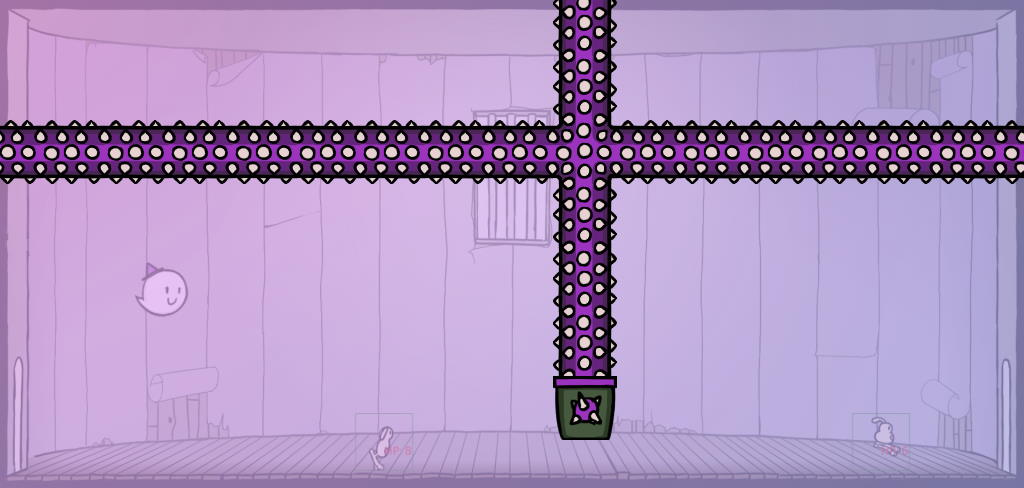
\includegraphics[scale=0.4]{images/eksempel.jpg}
            \caption{Concept for the purple cactus enemy}
        \end{figure}

    \subsection{Application pages}

        \subsubsection{The settings page}

        Originally, the plan was to let players adjust application settings and store them as settings configurations on the database. However, it seemd to overwhelming and unecessary to connect all the settings details to the game, such as adjusting display mode, audio and keyboard button mapping. The configuration model class is still in the model and the database, along with the settings page, but they are not fully implemented. I also realized I could have utilized the settings page from Windows Template Studio, but at that point I had moved on.

        \subsubsection{The spell book}

        Originally, the intent was that the player would have to memories combinations of button presses to fire spells. For example, the ice-spell would have a combo of up-up-down-down-up using the arrow keys, but I did not get to code it. This xaml page would give a listing of all the different button combinations required to initiate each spell. However, now it just rests in the main menu and serves no purpose.

\section{Known Issues}

\section{App Description}

    \subsection{General Information}

        \subsubsection{About the game}

        WizardGame is a small video game where players play as a tiny wizard ghost who can cast different spells. The objective is to survive as many waves of enemies as possible without dying, however this becomes more difficult as the waves progress. The enemy count and their damage output increases with the current wave, making it tougher and tougher to survive. 
        
        Another important place is the leaderboards. This is where players compete to get thee highest wave, crowning them as number one on the board. The list is ordered by each players personal best game in descending order. Players can also view their previous game to monitor their improvement.

        For this to be possible, each place have the ability to create their own player profile that store previous games, and will be displayed on the leaderboards. If they are unhappy with their decisions, they can update their player profile to give a more soothing name, or delete it alltogether.

        \subsubsection{Assets and cosmetic}

        All the textures and sprites for the game (items, characters, backgrounds, logo, etc) are drawn by me using digital editing software.

    \subsection{Functionality}

        \subsubsection{Gameplay}

        To move the ghost around use the W, A, S and D keys, and to cast spells use the up-, left-, down- and right-arrow keys. A wave progresses if all given enemies are eliminated. A normal wave consists of bunny enemies, and a special wave consists of card enemies and will occurr every ten waves. If a bunny or card enemy touches the ghost, the ghost will lose some health points. Once the health points reach zero, the game is over and it proceeds to save the game to the selected profile. 

        The arrow keys will cast different spells that are used to damage and evade the enemies. The most useful spell is the ice-spell (up-arrow) that shoots horizontaly in the headed direction and will deal a lot of damage to the enemies.

        \subsubsection{Application Pages}

        On launching the application, the user is greated with a titlescreen displaying the name. Press any button left-click to proceed to the main menu. From the main menu, it's immediately possible to navigate to the settings screen, player screen, and spell book screen. Only once the database connection has loaded in the viewmodel, do the leaderboards and game become available. During the main menu it is possible to play around with the ghost character.

        In the player page, users can select, create, update or delete any desired player profile. In the left panel, all existing players are displayed and ready to be handled by clicking on them. The selected player profile is each game will be tied to when playing. If no profile has already been selected, the rest api did not find a selected player, the application will instead select a default profile.

        The leaderboards page will list all players and their best game (highest wave) in descending order. This is also the page that lists a user specific games history, and can be found by using the pivot headers. The page only serves as a monitoring tool to track ones individual progress.
        
        The settings page and spell book page are not fully implemented.

\subsection{Screenshots / Concepts}

\begin{figure}[H]
    \centering
    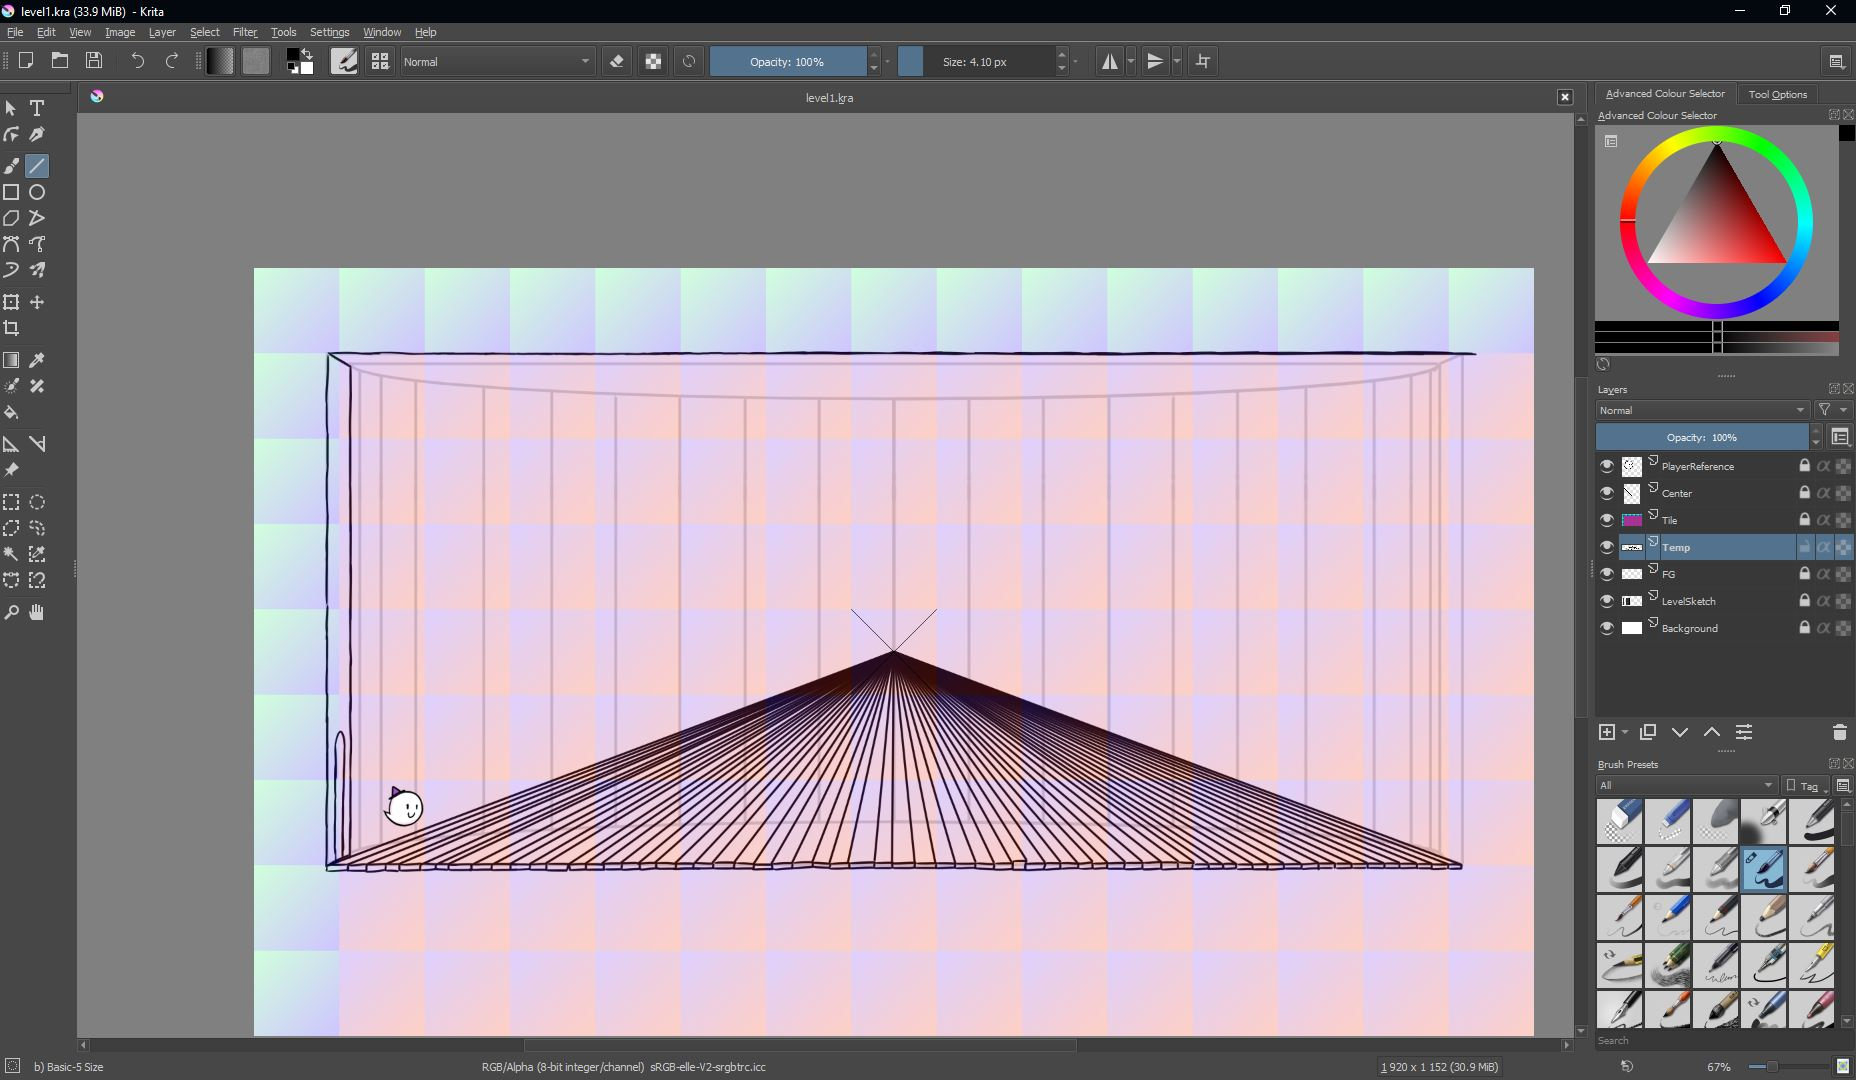
\includegraphics[max width=\textwidth]{images/002.JPG}
    \caption{Early draft on the level background}
\end{figure}

\begin{figure}[H]
    \centering
    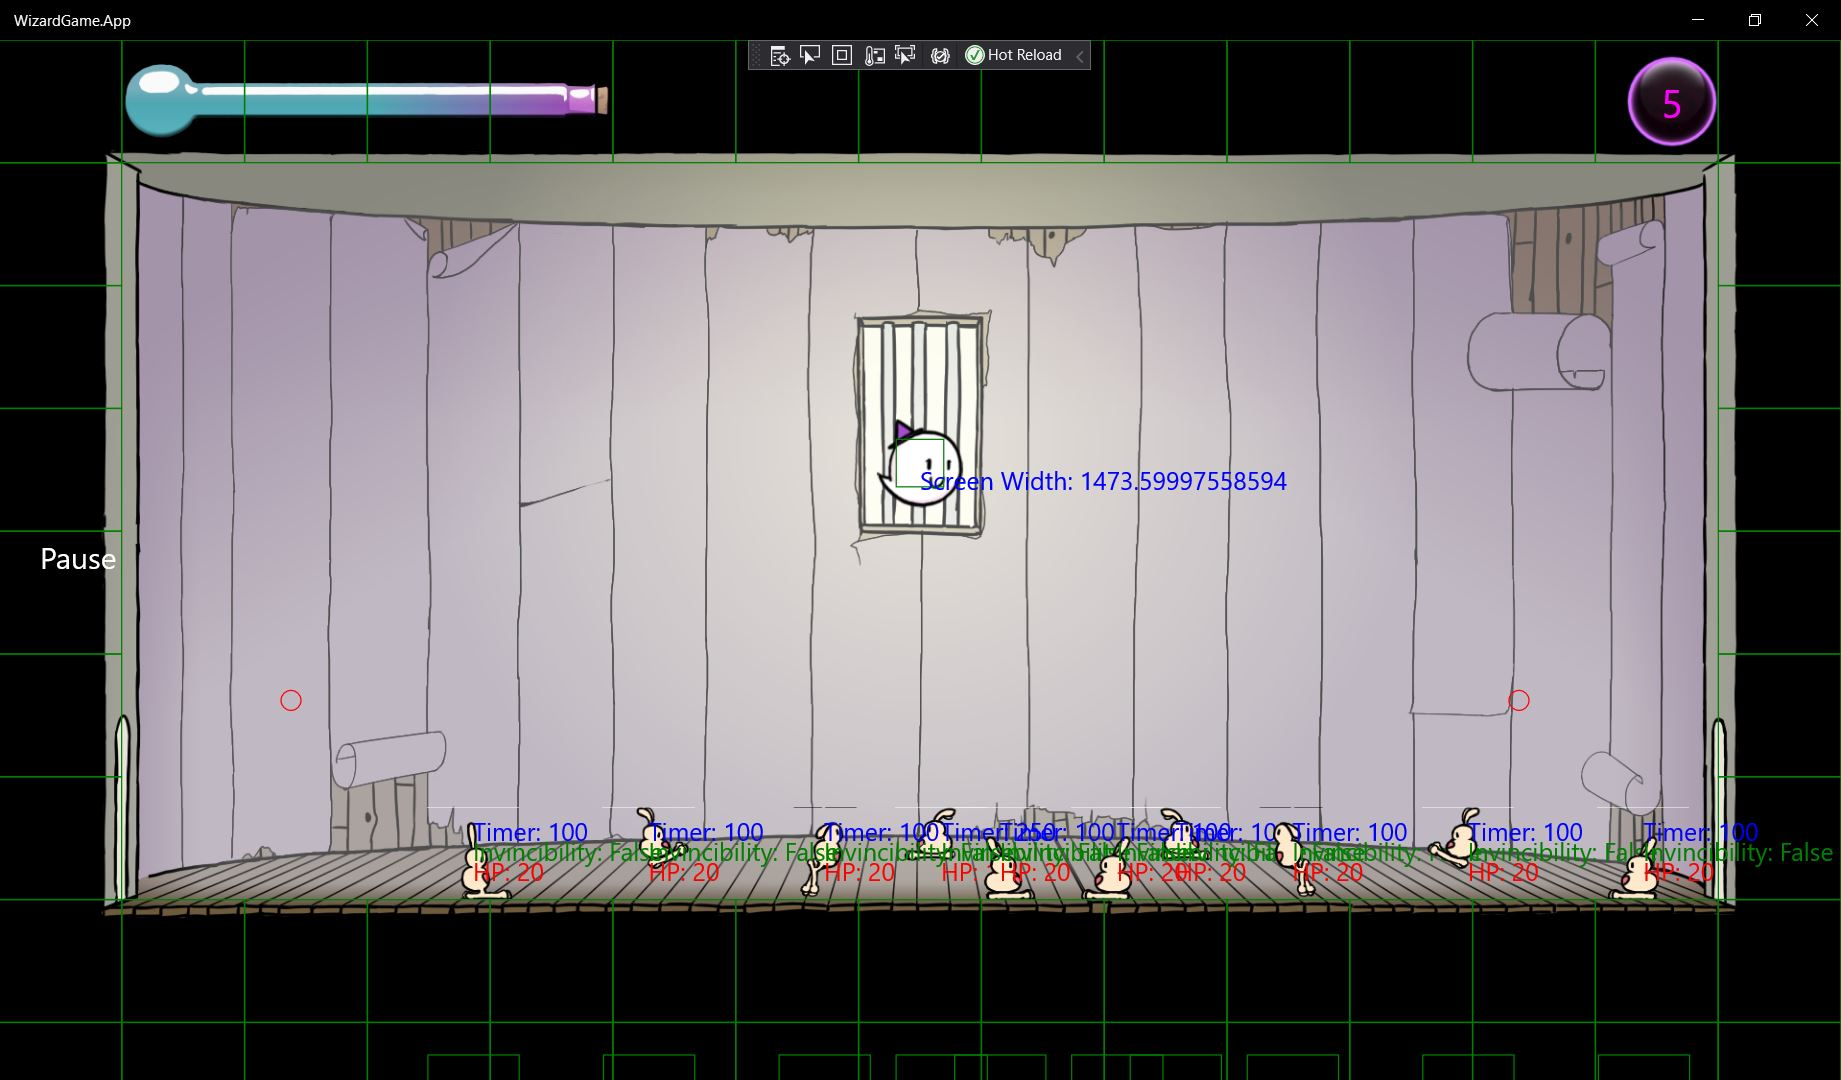
\includegraphics[max width=\textwidth]{images/019.JPG}
    \caption{Late development, displaying collision bounding-boxes}
\end{figure}

\begin{figure}[H]
    \centering
    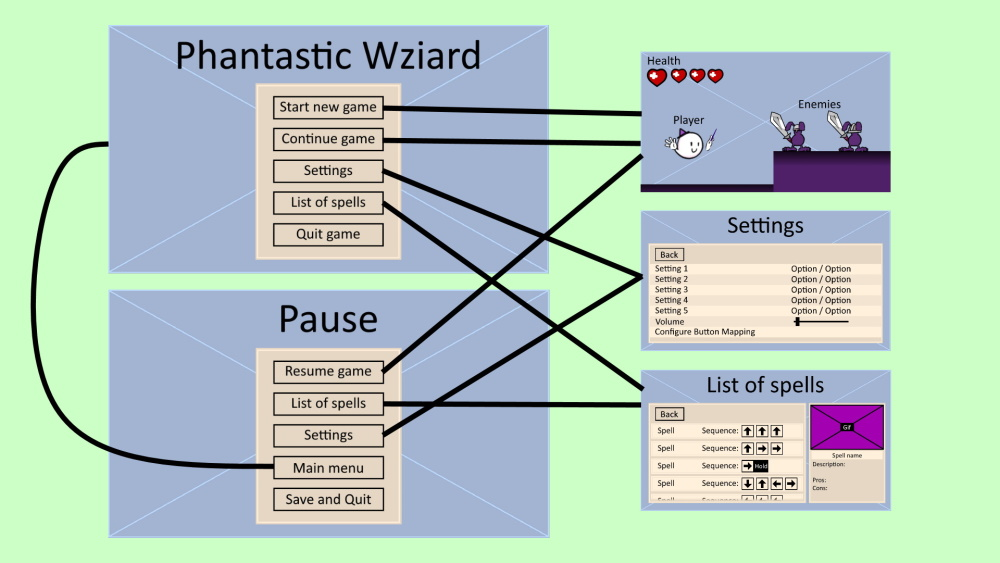
\includegraphics[max width=\textwidth]{images/menu_structure.jpg}
    \caption{Menu structure sketch}
\end{figure}

\begin{figure}[H]
    \centering
    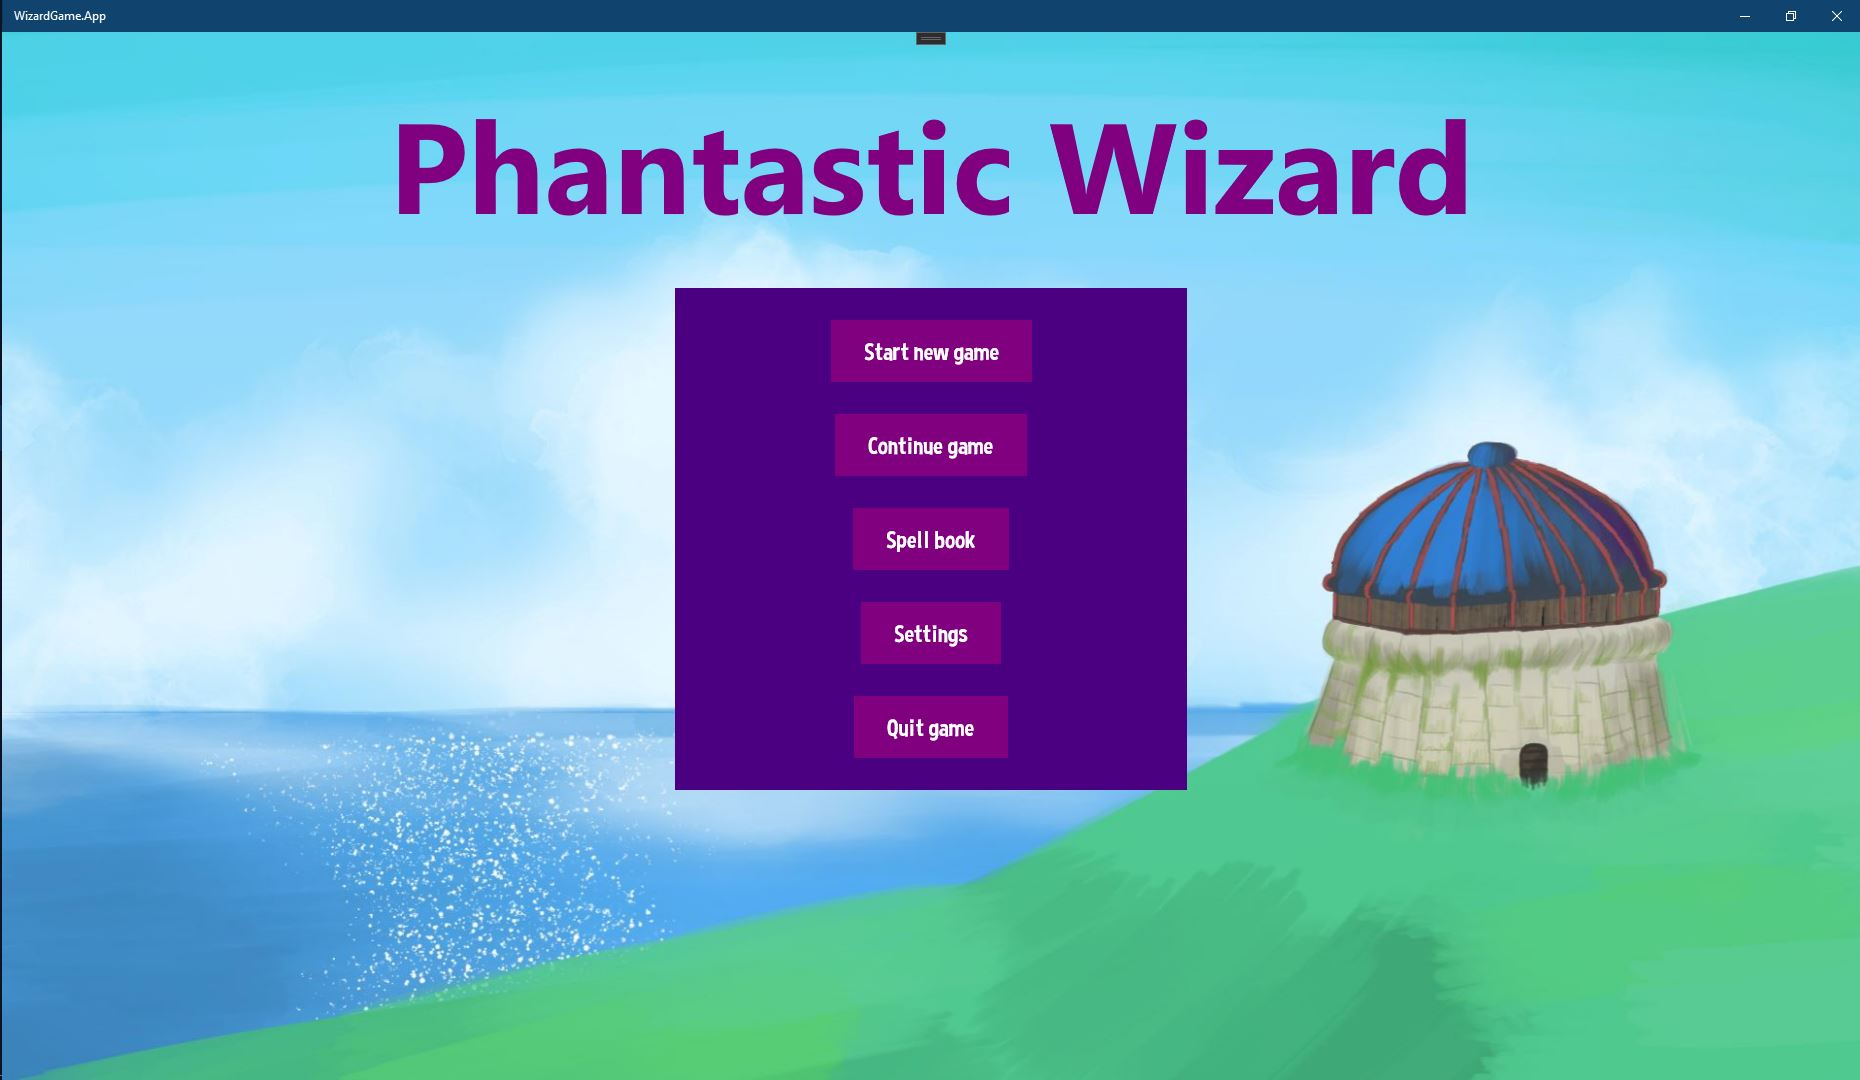
\includegraphics[max width=\textwidth]{images/013.JPG}
    \caption{First iteration of main menu}
\end{figure}







\end{document}